\chapter{Detector}\label{c:Det}

\section{The Large Hadron Collider}

	The Large Hadron Collider (LHC) is a circular particle accelerator operated at European Organisation for Nuclear Research (CERN, Conseil Europ\'{e}an pour la Recherche Nucl\'{e}aire). Currently the largest accelerator in the world, the LHC is designed to collide opposing beams of heavy ions or protons for a peak design \textit{centre-of-mass} energy $\sqrt{s}=14$TeV and a peak \textit{luminosity} of $10^{34}$cm$^{-2}$s$^{-1}$ \cite{lhc}. The first proton beams were circulated in the LHC in 2008, with Run-1 of LHC data taking being conducted until 2013, at which point the machine was shut down for scheduled maintenance. Following on from the long shut down period, Run-2 of the LHC has been ongoing since 2015, operating at $\sqrt{s}=13$TeV.

	The principle LHC ring consists of eight pairs of alternating long arc sections and short straight insertion sections, situated within the underground tunnel excavated for the older Large Electron Positron Collider experiment \cite{lep1, lep2}. The arc sections contain the dipole magnets used to bend the particle beam around the ring, while the straight sections contain four interaction points, at each of which the large experiments are located. The remaining straight sections contain the operational systems of the LHC: beam acceleration, injection,  dumping and collimation. The proton beams are generated outside the principle ring and inserted into the ring by the LHC injector chain, a sequence of smaller accelerators which are used to bring the proton beams up to a suitable energy for injection.The proton beams injected into the accelerator originate from a cloud of hydrogen gas, which is passed through an electric field to strip the electrons before the protons are inserted into the beam acceleration components. The proton beams are arranged such that the protons move in bunches of $\mathcal{O}(10^{11})$ protons, with multiple bunches placed into trains. During Run-2 the LHC operated with bunch spacings of $50$ns and $25$ns between the bunch trains.

	The principle measure of the operation of the LHC is the beam luminosity, expressed as either instantaneous luminosity $L$ or an integrated luminosity. This parameter is a measure of the rate of collisions within the accelerator, given by:

	\begin{equation}
		L = \frac{1}{\sigma}\frac{dN}{dt} = \frac{n_bn_1n_2f}{2\pi\Sigma_x\Sigma_y}
	\end{equation}

	where in the general case $\sigma$ is the interaction cross section and $\frac{dN}{dt}$ is the event rate. In the LHC specific formula, $n_b$, $n_1$ and $n_2$ are the number of bunch crossing producing collisions, and the number of bunches in both of the colliding beams, $f$ the machine revolution frequency, and $\Sigma_{x, y}$ are parameters relating to the beam width. This instantaneous luminosity is integrated across a time period, such as an LHC Run or a specific data period, to produce the integrated luminosity $\int L dt$ which is a measure of the total recorded data.

	Once a beam is accelerated to the target energy collisions begin at the interaction points. Interactions are ongoing for periods of several hours, and will go on until the the beam is replaced due to general decay of the interaction rate or beam instabilities.

	At the LHC, the four large experiments at the interaction points are ATLAS (A Toroidal LHC ApparatuS), CMS (Compact Muon Solenoid), LHCb (LHC beauty) and ALICE (A Large Ion Collider Experiment). LHCb is a forward spectrometer heavy flavour experiment, designed to study flavour physics with emphasis on the \bquark and on matter/anti-matter asymmetry. ALICE focuses on the collisions of heavy ions, while ATLAS and CMS are general purpose detectors to conduct experiments across a broad range of modern physics research areas.

	\subsection{Run Conditions in 2016}

	Over the course of 2016, following beam commissioning runs, the LHC beam was operated predominantly with two beams of energy $6.5$TeV for $\sqrt{s}=13$TeV. Over the course of the 2016 data-taking the ATLAS and CMS experiments achieved an integrated luminosity of $40$ fb$^{-1}$ with a peak instantaneous luminosity of $1.4\times10^{34}$cm$^{-2}$s$^{-1}$ with 2220 bunches per beam \cite{Run2016}.


\newpage
\section{The ATLAS Detector}

	The ATLAS detector \cite{ATLAS} is a multi-purpose detector designed to study a broad selection of physics phenomena within the experimental conditions of the LHC. The detector is cylindrical in structure with the axis aligned to the beam path and nominally forward-backward symmetric in terms of the beam collision point at the centre of the detector. The detector provides approximately $4\pi$ solid angle coverage around the interaction point to detect as many collision products as possible.

	The structure of the ATLAS detector is composed of concentric subsystems around the interaction point.  The Inner Detector (ID) is the component closest to the interaction point, and is contained in a superconducting solenoid. This is surrounded by high-granularity calorimeters and an extensive muon spectrometer contained within an eight-fold azimuthally symmetric arrangement of three large toroidal magnets. A schematic representation of the ATLAS detector is shown in Figure \ref{fig:t:ATLAS}. 	The subsystems are arranged into three cryostats, two \textit{endcaps} located on the ends of the detector and the central \textit{barrel} section. Discussion of the coordinates and quantities used in the detector is found in Section \ref{t:geometry}. A summary of the operational parameters of the principle detector components is given in Table \ref{tab:d:operational}.

	\begin{figure}[h]
		\centering
		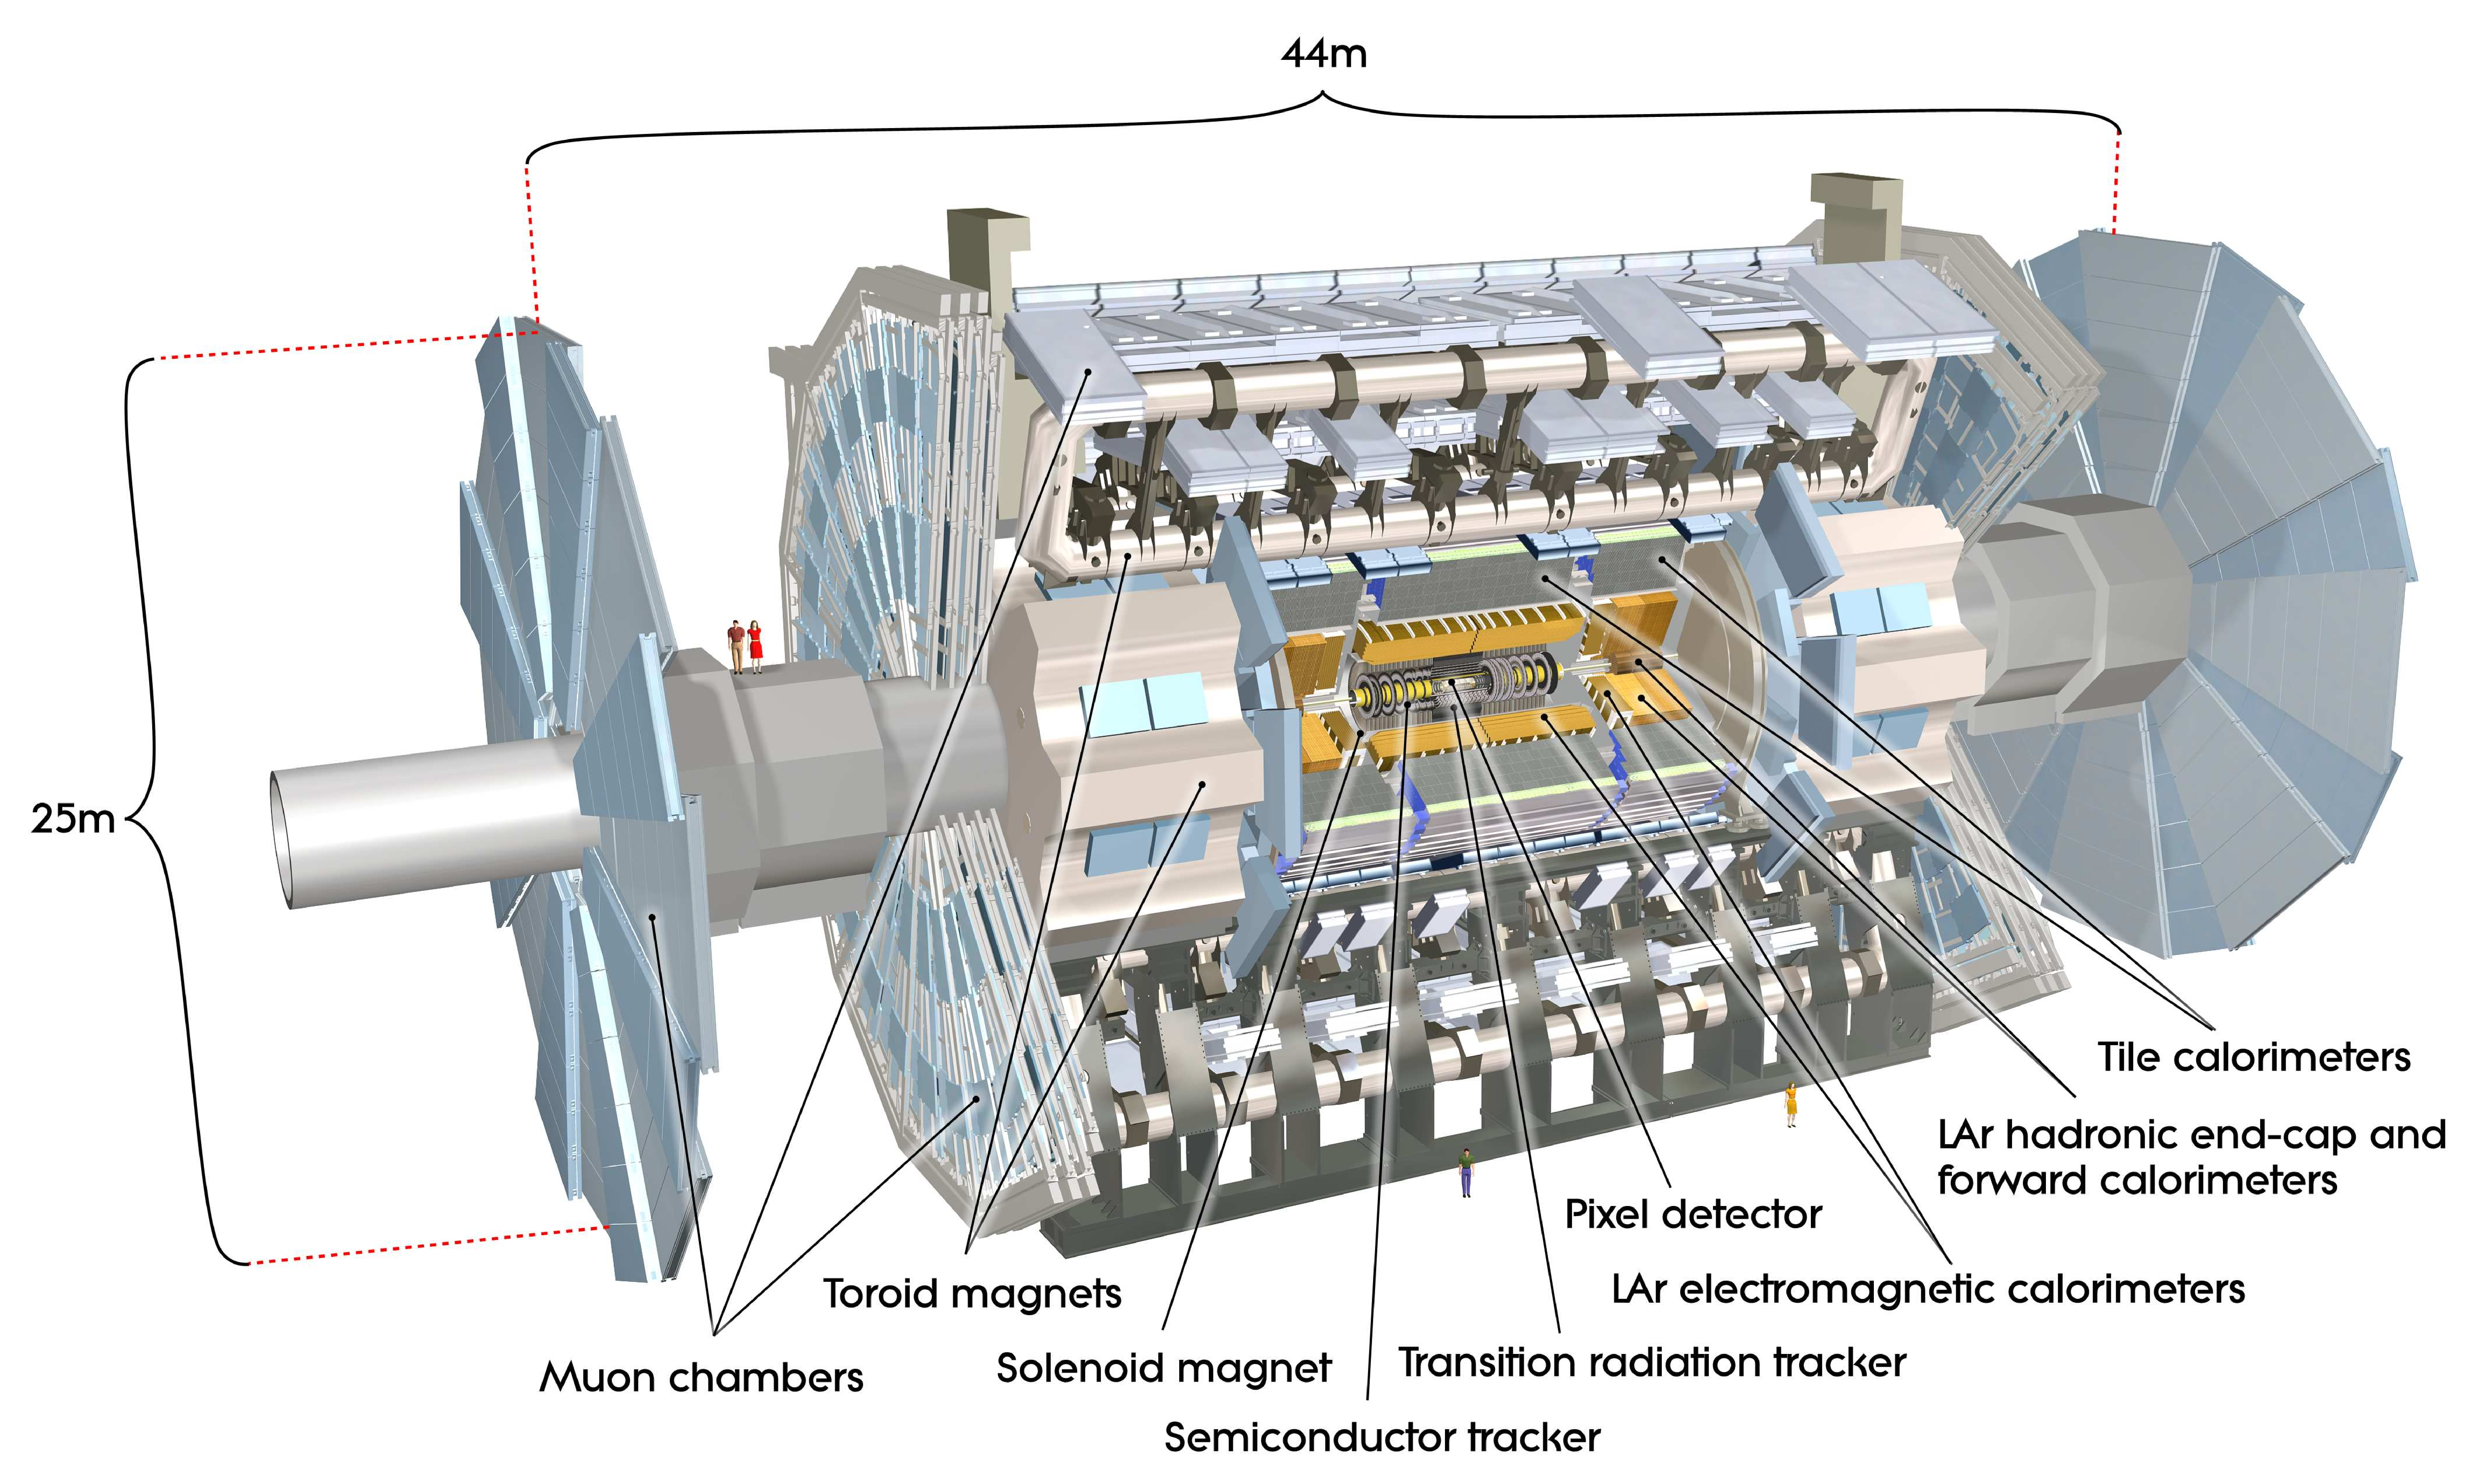
\includegraphics[width=0.7\linewidth]{D/FIGS/ATLAS_SE_Corrected7}
		\caption{Schematic cut-away of the ATLAS detector \cite{ATLASSchem}.}
		\label{fig:t:ATLAS}
	\end{figure}

	The conventional coordinate system used to describe the detector takes the interaction point as the origin, with $x$ pointing horizontally out into the detector, $y$ out and upwards with $z$ along the direction of the beam line. The angle $\phi$ describes azimuthal rotation around the beam pipe and as discussed in Section \ref{t:geometry}, $\theta$ is the polar angle along the beam line.


	\subsection{Inner Detector}
	\label{d:id}

		The Inner Detector provides pattern recognition, momentum measurements, electron identification and measurements of both primary and secondary vertices to efficiently identify jets containing \bhadron within a pseudorapidity range $|\eta|<2.5$. The ID itself is contained within a 2 T solenoidal field, which is used to bend the paths of charged particles within the ID. The ID is specifically designed to have a high momentum resolution (Table \ref{tab:d:operational}), and consists of three separate detector sections: the silicon pixel detector provides fine granularity track and vertex reconstruction, the silicon strip semiconductor tracker measures the trajectory of transiting charged particles and the outer transition radiation tracker used for particle identification is comprised of layers of straw tubes containing mixtures of xenon, oxygen and carbon dioxide.

	\subsection{Calorimeters}

		Calorimeters are used to measure the energy of any particle moving out from the interaction point. These particles cause the development of either electromagnetic (EM) or hadronic showers within the calorimeter substrate, and the energy deposited in this shower can be used to calculate the energy of the incoming particle. The ATLAS calorimetry system consists of a combination of EM and hadronic calorimeters arranged with full $\phi$-symmetry around the beam axis. The combination of all separate calorimeters provides pseudorapidity coverage in the range $|\eta| < 4.9$. Within the pseudorapidity region of the inner detector, the fine granularity of EM calorimeters is optimised for measurements of electron and photon tracks and momenta, while the coarser hadronic calorimeters contained in the remainder of the calorimeter system are sufficient for jet reconstruction and missing energy calculations. The structure and design of the calorimeter components has been optimised to provide complete azimuthal coverage, take into account the engineering requirements for assembling the detector and account for radiation considerations between the different detector components \cite{ATLAS}.

		The EM calorimeter is a lead-Liquid-Argon (LAr) detector, which is split into a barrel section (EMB, $|\eta|<1.475$) and two endcap sections (EMEC, $1.375<|\eta|<3.2$) with each section contained in a separate cryostat. The EMB consists of two identical half-barrels split by a small gap at $z=0$. Each of the EMEC sections is a pair of coaxial wheels, with the inner and outer sections covering regions $1.375<|\eta|<2.5$ and $2.5<|\eta|<3.2$ respectively. The major body of the EM calorimeter is divided into 3 sections of decreasing cell granularity, moving out from the beamline.

		Hadronic calorimetry for particles undergoing the strong interaction is provided by the steel/scintillator tile calorimeter for pseudorapidity values of $|\eta|<1.7$, and by the LAr flat-plate Hadronic Endcap Calorimeter (HEC) for $1.5<|\eta|<3.2$. The tile calorimeter directly surrounds the EM calorimeter, and is split into a central barrel section for $|\eta| < 1.0$ and two extended barrel sections covering $0.8<|\eta|<1.7$. The HEC, akin to the EMEC, consists of two separate wheels per end-cap covering $1.5<|\eta|<3.2$, and is contained within the same cryostat as the EMEC. The HEC consists of alternating copper plates with LAr gaps to act as the active medium.

		In addition to the barrel and end-cap calorimeters, the LAr Forward Calorimeter is contained within the end-cap cryostat (The FCal is omitted from Figure \ref{fig:t:ATLAS}) and is designed to perform both EM and hadronic calorimetry across a pseudorapidity range of $3.1<|\eta|<4.9$ using a combination of copper/LAr (EM) and tungsten/LAr (hadronic) calorimeter components.

	\subsection{Muon Spectrometer}

		The muon spectrometer is the outermost component of the ATLAS detector, measuring trajectory and momentum of muons from the interactions within a pseudorapidity range of $|\eta| < 2.7$. The muon system consists of three large superconducting coils that deflect the muon trajectories. The system is designed for high precision tracking of the minimally ionising muons and for use in the triggering system.


	  	\begin{table}[ht]
	  		\caption{Performance goals and operational ranges for thr principle components of the ATLAS detector. \cite{ATLAS}}
	  		\label{tab:d:operational}
	  		\medskip
	  		\centering
	  		\begin{tabular}{llll}\toprule
	  			System & Component & $\eta$ Coverage & Resolution \\\midrule
	  			Tracking &  & $0<|\eta|<2.5$ & $\sigma_{p_\text{T}}/p_\text{T} = 0.05\% p_\text{T}\oplus1\%$\\
	  			EM Calorimetry & EMB & $0<|\eta|<1.475$ & $\sigma_{E}/E = 10\%/\sqrt{E} \oplus0.7\%$ \\
	  			& EMEC (Inner) & $1.375<|\eta|<2.5$ &  \\
	  			& EMEC (Outer) & $2.5<|\eta|<3.2$ &  \\
	  			Hadronic Calorimetry & Tile (Barrel) & $0<|\eta|<1$ & $\sigma_{E}/E = 50\%/\sqrt{E} \oplus3\%$ \\
	  			& Tile (Extended) & $0.8<|\eta|<1.7$ &  \\
	  			 & HEC & $1.5<|\eta|<3.2$ &  \\
	  			Forward Calorimetry & FCal & $3.1<|\eta|<4.9$ & $\sigma_{E}/E = 100\%/\sqrt{E} \oplus10\%$ \\
	  			Muon Spectrometer &  &  $0<|\eta|<2.7$  & $\sigma_{p_\text{T}}/p_\text{T} = 10\%\,at\,p_\text{T}=1$ TeV  \\\bottomrule
	  		\end{tabular}\\[5pt]
	  	\end{table}

\section{Triggers}

	When operating at the design luminosity, the LHC produces a bunch-crossing rate of 40 MHz \cite{trigrun2017}. This extreme rate of interaction necessitates a trigger system to reduce the output rate to a suitable level for offline processing, which is predominantly limited by the rate at which data can be written to disk. The trigger system selects events by quickly identifying distinguishing features of events, signatures of muons, electrons, jet and \bjet objects, and using combinations of these signatures to signify an event as relevant for further analysis. Overall usage of the trigger system brings the output rate down to 1 kHz with a maximum Level 1 trigger (L1) rate of 100 kHz.

	The ATLAS trigger system consists of a chain of selection stages of increasing severity and corresponding decrease in rate. A schematic outline covering both the logical process and the transfer of data between components of the trigger chain is shown in Figure \ref{fig:trigschem}. The principle decision logic of the trigger system is contained in two sections, the L1 trigger sytem and the High Level Trigger (HLT).

	\begin{figure}
		\centering
		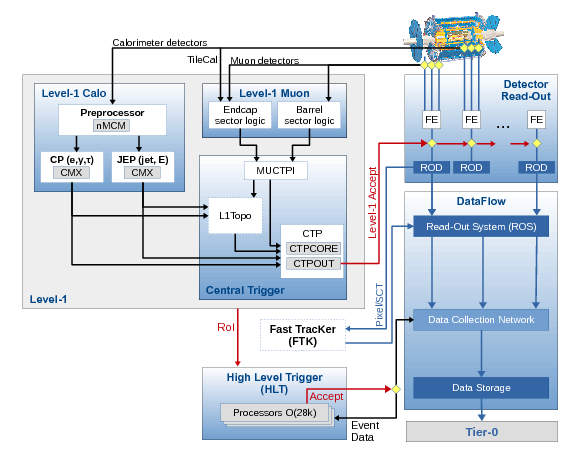
\includegraphics[width=0.8\linewidth]{D/FIGS/trigschem}
		\caption{Schematic plot of the ATLAS Trigger and Data acquisition system \cite{trig2015}.}
		\label{fig:trigschem}
		\end{figure}

	The L1 trigger system \cite{L1} is a hardware based decision system, using fast custom electronics to minimise latency in any decision. The L1 uses reduced-granularity data from the calorimetric and muon detectors, reconstructed objects and missing and total transverse energy. The high bunch-crossing rate means instantaneous processing of the event is non-viable, so event readouts are stored in a buffer chain of events to be evaluated with a fixed permitted decision time per event. Along with this first selection, the L1 trigger defines \textit{Regions of Interest} (RoIs) in the phase space within the detector, which are labeled for investigation in the HLT.

	In contrast to the hardware computation of the L1 system, the HLT consists of software algorithms running in a farm  of $\approx40000$ interconnected processors \cite{trigrun2017}. Following acceptance of an event by the L1 trigger, events are transferred from the initial data pipeline to dedicated readout buffers for the HLT. The HLT performs processing on the events using finer-granularity information from the calorimeters and muon spectrometer, along with making use of information from the ID, which is unavailable to L1. This more precise data is then computed using object reconstruction algorithms to generate particle objects similar to the objects reconstructed at a later point the data has been stored. The decision at HLT level to store an event is managed by a trigger chain, which is a sequence of specific criteria and algorithms evaluated on an event in sequence.

	A key component of the trigger chain is the prescaling factor of the chain; if the particular event requirements are not tight cuts, the overall output rate of the trigger chain is reduced by the prescale factor to bring the output rate within bandwidth limits. The HLT provides $\mathcal{O}(1000)$ independent trigger chains for evaluating events. Along with the partial reconstruction of relevant objects, the HLT is capable of performing complete reconstruction of an event, and also capable of writing out these partial or complete reconstructions of an event into different data streams from the complete detector readout for use in analysis. The standard terminology for events and data recorded and processed during the operation of the LHC is \textit{online} data, while objects and information produced by considering the output of the detector after the data has been stored is termed \textit{offline}. These terms are used extensively throughout the rest of this analysis to distinguish between the different data sources.

\section{Event Selection}

	Beyond the reduction in event storage handled by the trigger chains and prescaling, only select sections if the overall output dataset are ever used in analyses. The LHC is not free from operational errors or issues with the hardware and software of the detector. Parts of the output data can be corrupted by incomplete events due to detector failings, poor data integrity or disruption of the machine. From the complete output for a Run section, which is divided into luminosity blocks, only the blocks which have been marked as \textit{good} are made use of in analyses. The internal directory of usable luminosity blocks is named the Good Runs List (GRL).

	Along with these event selections based on using correct data, analyses typically refine events down to a particular area of focus, which is discussed for this analysis in Chapter \ref{c:ES}.

\newpage
\section{Object Reconstruction}

	\subsection{Jets}

	As discussed in Section \ref{t:hadronisation} the coloured fragments produced during collisions result in collimated streams of hadrons called jets, which are the physical objects detected in the event. Detectors make use of algorithms to reconstruct these jets from the calorimeter readouts to relate the stream of hadrons to the initial fragmented partons. There are various algorithms used to reconstruct jets within the ATLAS detector, and these algorithms commonly require the definition of a jet to be invariant under additional soft or collinear emissions. Such algorithms are designated as infra-red (IR) or collinear (C) safe.

	Modern jet algorithms are broadly split into two types: cone-type and sequential clustering algorithms. Cone-type algorithms take the hardest (highest momentum) object in an event as a seed of an iterative process of looking for a stable cone rooted at this seed \cite{cone-type}. Once a cone is defined, any constituents contained within the cone are removed from consideration and the process repeats. The alternate sequential clustering algorithms assume that particles within jets will have small differences in transverse momentum and groups particles based on the momentum space to reconstruct the jets. Sequential clustering algorithms function using iterative steps with two distance parameters. The first distance is the separation between two particles:

	\begin{equation}
		d_{ij} = min(p_{\text{T}i}^a, p_{\text{T}j}^a)\frac{\Delta R_{ij}^2}{R}
	\end{equation}

	where $a$ is a particular exponent for a given algorithm, $R$ is the radius parameter of the final reconstructed jet size and $\Delta R_{ij}$ is the ($\eta, \phi$) space distance between the two objects. The second parameter $d_{iB}$, is the momentum space distance between the beam axis and an object \cite{jetreco}:

	\begin{equation}
	d_{iB} = p_{\text{T}i}^a
	\end{equation}

	The principle algorithm used for jet reconstruction at ATLAS is the anti-$k_t$ algorithm \cite{antikt}, which is a sequential clustering algorithm with $a=-2$. The algorithm is seeded with the highest \pt particles in the event, and iteratively computes both distance parameters. At each step, the two are compared: if $d_{ij}$ is smaller, particles $i$ and $j$ are combined whereas if $d_{iB}$ is smaller particle $j$ is labeled as a jet. The fact this algorithm tends to result in approximately circular reconstructed jet objects makes it favourable for modern analyses. The sequential clustering algorithms are in addition theoretically preferable, but were impractical until recent advancements in the algorithms gave significantly increased computational performance. The anti-$k_t$ algorithm is IRC safe and typical used with $R=0.4$ in the ATLAS experiment, and can be readily applied to clustering partons and calorimeter deposits in addition to hadrons.

	During jet reconstruction, when the energy deposits are extracted from the calorimeter, there is the option of reading the calorimeter cells according to the Electromagnetic (EM) scale, which is calibrated using test electron beams, or by applying Local Cell (LC) corrections to account for the attenuated physical response of the calorimeter and the difference in hadronic and electromagnetic response, which restores the energy of extracted objects to correspond to Monte-Carlo simulated truth objects. In this analysis, readouts of all jet objects, both offline and trigger level, were taken at the EM energy scale.

	\subsubsection{Pileup}

	As mentioned in Section \ref{t:underlying} on the process of a $pp$ collision, there are significant interactions as a result of the parton interactions accompanying the hard-scatter interaction of the collision. These lower \pt collisions produce additional jets and objects that contaminate the signal collision. The collection of these jets in the detector output is termed in-time pileup. In addition to the jets from the underlying event, interactions from preceding or subsequent bunch crossings also contribute contaminating objects to the detector readout, which is named out-of-time pileup. In-time and out-of-time pileup are collectively referred to as pileup in the detector, and necessitate processing and calibration of the detector output to remove the effects from consideration \cite{pileup}.

\subsection{\textit{b}-Tagging}
\label{det:btagging}

	Identification of \bquark jets in ATLAS is based on combining the output of three separate \btag algorithm types: Impact Parameter based algorithms (IP2D and IP3D, Section \ref{det:btag:ip}), Secondary Vertex based (SV, Section \ref{det:btag:sv}) and Decay Chain based (JetFitter, Section \ref{det:btag:jf}) into a multivariate discriminant (MV2, Section \ref{det:btag:mv}) which is used to distinguish the jet flavours. These algorithms have undergone continuous improvement over the Run-2 cycle of the LHC to improve the separation of jet flavours.

	The inputs for each of the \btagging algorithms are all taken from the ID of the ATLAS detector (Section \ref{d:id}). This limits \btagging to jets with $|\eta|<2.5$, and in addition jets with a \pt$<20$GeV are not selected for \btagging, nor jets determined to be likely a result of pileup in the detector which are eliminated using a multivariate discriminant from Jet Vertex Tagger algorithm \cite{btagOptimisation, pileup}.

	\subsubsection{IP2D and IP3D: Impact Parameter based Algorithms}
		\label{det:btag:ip}

		The typical topology of a \bhadron; a secondary vertex displaced from the hard scatter interaction point as a results of the lifetime of \bquark, is used as the basis of these algorithms. Impact parameters of tracks from the secondary vertex are computed with respect to the primary vertex of the interaction. The IP2D algorithm uses a transverse impact parameter $d_0$ defined as the distance of closest approach of a track to the  primary vertex in ($r$, $\phi$) plane around the vertex. The IP3D algorithm uses both the transverse impact parameter and a correlated longitudinal impact parameter $z_0\sin\theta$, defined as the distance between the point of closest approach in ($r$, $\phi$) and the primary vertex in the longitudinal plane. These parameters typically have large values as a result of the lifetime of \bquark. The signs of the impact parameters are also defined to take account of if they lie in front or behind the primary vertex with respect to the jet direction, with secondary vertices occurring behind the primary vertex normally due to background.

		The significance of the impact parameter values ($\frac{d_0}{\sigma_{d_0}}$, $\frac{z_0}{\sigma_{z_0\sin\theta}}$) for each track are compared to probability density functions obtained from reference histograms derived from Monte Carlo simulation, with each track being compared to a selection of reference track categories. This results in weights which are combined using a log-likelihood ratio (LLR) discriminant to compute an overall jet weight separating the $b$, $c$, and light-jet flavours from each other. \cite{btagOptimisation, bTagPerformance}

	\subsubsection{SV1: Secondary Vertex Finding algorithm}
	\label{det:btag:sv}

		The secondary vertex algorithm uses the decay products of the \bhadron to reconstruct a distinct secondary vertex. The algorithm uses all tracks that are significantly displaced from the primary vertex associated with the jet, forming vertex candidates for all pairs of track, while rejecting any vertices that would be associated with decay of long lived particles (e.g. $\Lambda$, $uds$), photon conversions or interactions with the material in the detector. The tracks forming these vertex candidates are then iteratively combined and refined to remove outliers beyond a $\chi^2$ threshold leaving a single inclusive vertex.

		The properties of this secondary vertex are used to differentiate the flavour of the jet. The SV1 algorithm is based on a LLR formalism similar to the IP algorithms, and makes use of the invariant mass of all charged tracks used to reconstruct the vertex, the number of two track vertices and the ratio of the invariant mass of the charged tracks to the invariant mass of all tracks. In addition the algorithm is signed in a similar fashion to the IP algorithms and uses the $\Delta R$ between the jet direction and secondary vertex displacement direction in the LLR calculation. The algorithm uses distributions of these variables to distinguish between the jet flavours \cite{btagOptimisation, bTagPerformance}.

	\subsubsection{JetFitter: Decay Chain Multi based Algorithm}
	\label{det:btag:jf}

		The JetFitter algorithm exploits the topological structure of weak \bhadron and \chadron decays inside the jet to reconstruct a full \bhadron decay chain. A Kalman filter is used to find a common line between the primary, \bhadron and \chadron vertices to approximate the \bhadron flight path \cite{jetfitter}. A selection of variables relating to the primary vertex and the properties of the tracks associated with the jet are used as input nodes in a neural network. This neural network uses the input variables, \pt and $|\eta|$ variables from the jets, reweighted to ensure the spectra of the kinematics are not used in the training of the neural net. The neural network outputs discriminating variables relating to each jet flavour which are used to tag the jets. \cite{btagPerformance}

	\subsection{Multivariate Algorithm}
	\label{det:btag:mv}

	The output variables of the three basic algorithms described prior are combined as input into the Multivariate Algorithm MV2. MV2 is a Boosted Decision Tree (BDT) algorithm which has been trained on $t\bar{t}$ events to discriminate \bjets from light and \cjets. The algorithm makes use of the jet kinematics in addition to the tagger input variables to prevent the kinematic spectra of the training sample from being used as discriminating factor. The MV2 algorithm is an revised version of the MV1 algorithm used during Run-1 of the LHC, and has three sub-variants (MV2c00, MV2c10, and MV2c20) of the algorithm distinguished by the exact background composition of the training sample. The naming convention initially referred to the \cjet composition of the training sample; for MV2c20 the \bjets are designated as signal jets where a mixture of 80\% light jets and 20\% \cjets was designated as background.

	The MV2 algorithm has a set of working points, defined by a single value of the output distribution of the algorithm, which are configured to provide a specific \bjet selection efficiency on the training $t\bar{t}$ sample. Rather than being used independently, physics analyses will make use of several working points as an increase in \bjet efficiency (corresponding to \textit{looser} \bjet selection) will bring an increased mistag rate of light and \cjets.

	These algorithms were refined prior to the 2016 Run-2 data-taking session in response to \cjets limiting physics analyses more the light-jets. This change  to enhance the \cjet rejection meant that for the MV2c10, the \cjet fraction was set to 7\% in training and the fraction for MV2c20 was 15\%. There were a selection of other improvements made to the algorithm relating to the BDT training parameters and the use of the basic algorithms before the 2016 data taking. With these refinements, the MV2c10 algorithm was found to provide a comparable level of light-jet rejection to the original 2015 Mv2c20 algorithm with improved \cjet rejection, so was chosen as the standard \btag algorithm for 2016 analyses. \cite{btagOptimisation}


\section{Trigger-Object Level Analysis}

	In physics analyses at the LHC, the $1$kHz event readout rate to storage is significantly below the $40$MHz bunch crossing rate. This bottleneck is caused by the limited bandwidth (event rate $\times$ event size in bytes) available to analysis channels. In searches with large backgrounds or those with low rates, the prescaling introduced in the trigger system critically effects the amount of significant events output to storage, limiting the statistical power of any search in these hard to isolate channels as a large number of events are discarded to keep output within bandwidth limitations.

	This constraint can be alleviated by recording only a fraction of the detector readout for any given event, specifically the jet information reconstructed by the triggering system. This partial event corresponds to a reduction in the event size in bytes which allows for present bandwidth limitations to be upheld with an increased event rate. This process of using the objects produced in the trigger as substitutes for the offline objects is referred to as Trigger-Object Level Analysis (TLA) \cite{tla}.

	In these analyses, partially built events are collected using an additional TLA stream of the output data, which records the jet four-momentum along with a selection of additional identifying variables for jet objects in the HLT, triggered by jet objects from the L1 trigger. The readout does not include individual calorimeter cells nor information from the muon or tracking detectors, and in prior application of a TLA approach to a search for light dijet resonances \cite{tla} a partial TLA event was $~5\%$ of the size of a full detector readout.




\endinput
